\chapter{Background}\label{chap:background}
\section{Architecture}
The architectures shown below describes how communication between Project Recon and the general interface would look like. Figure 3.1 shows more details regarding the internal architecture and design of Project Recon itself.
\\
\\
As shown in figure~\ref{projectrecondiagram}, Project Recon main inputs are the Kinect sensor and Thai Pad Sensor. The Kinect sensor sends the Image stream and skeleton stream to Project Recon's Technique recognizer which in turn would take the skeleton of the user and keep track of its joints' position in time. When the practitioner moves the technique recognizer would compare the current movement with the database of reference moves. From this, it would associate the detected move with its respectful reference. The sensor equipped Thai Pads would measure the impact and send the value to Project Recon. The impact is then linked to its respectful technique and compared with reference impact. All this data is sent to the client which is responsible for the connection between the interface and Project Recon.
\begin{figure}[htb]
\centering
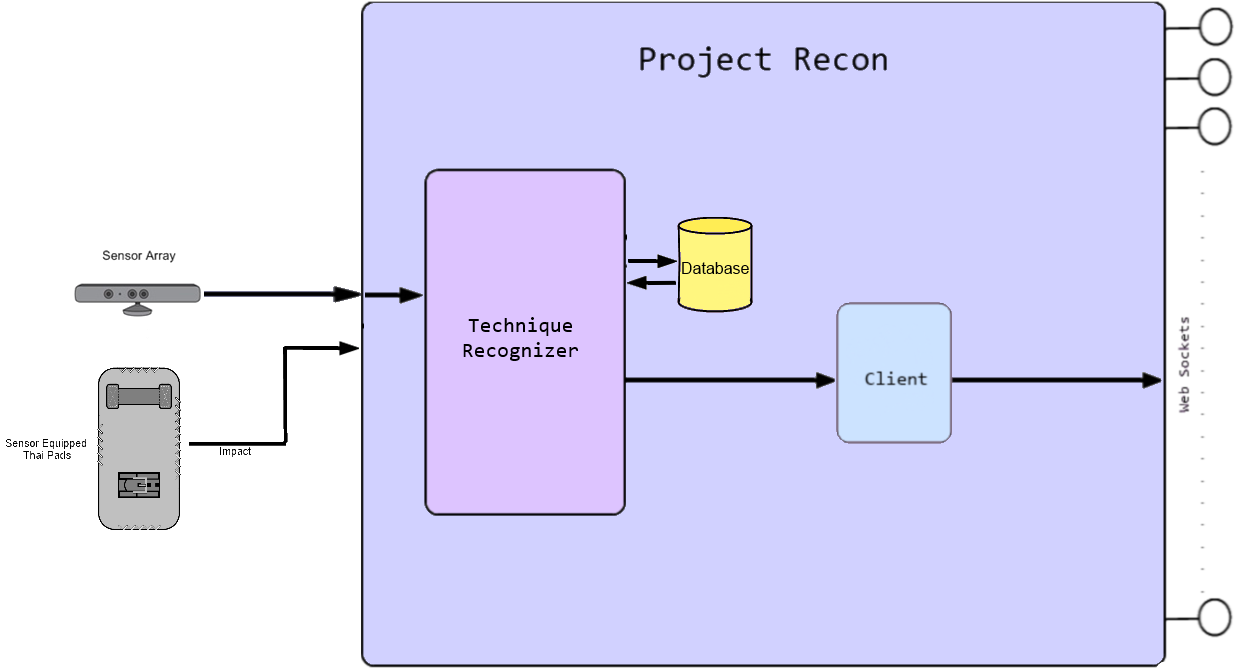
\includegraphics[width=1\textwidth]{images/project_Recon_diagram.png}
\caption{Internal architecture and design of Project Recon}
\label{projectrecondiagram}
\end{figure}
\\
\\
In figure~\ref{generaloverview}, an overview of the project is shown. Where it shows the linking between the Main Interface and Project Recon. As previously said, the client is responsible for the connection between both by communicating and connecting to a socket specified for it by the Main Interface.
\begin{figure}[ht]
\centering
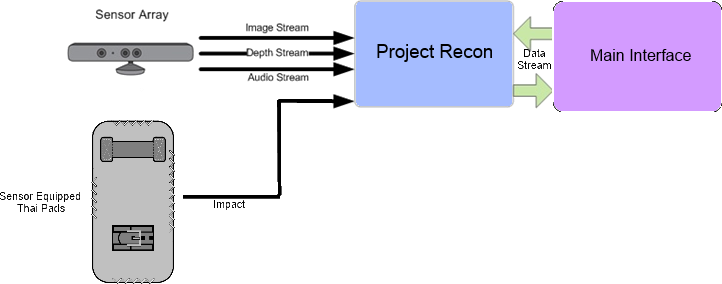
\includegraphics[width=1\textwidth]{images/general_overview.png}
\caption{Overall architecture of Project Recon and its connection to the interface}
\label{generaloverview}
\end{figure}
\section{Development Tools and Technologies}
When it came to developing with Kinect, two choices were on the table. Whether to use the official Microsoft Kinect SDK or use other unofficial SDK's. The official Kinect SDK may have slightly less capabilities, and we will be talking about them later and exploring them more. However, it is easier to use the official Microsoft SDK. The environment that was chosen for development (XNA) would also support our choice of using the official SDK. The programing language possible to use are Visual Basic and C\#. The chosen language was C\# as it was easier for me to develop for.

\subsection{Microsoft XNA}
XNA is an IDE (Integrated Development Environment) created by Microsoft to help game development for their systems to be easier. XNA is based on .NET Framework and it creates applications for platforms like XBox 360, Zun, Windows Phone and Microsoft Windows. Since its release there are 4 versions with the final version being XNA Game Studio 4.0. The framework was released on March of 2004 and the latest update released on September 16th 2010.
\\
\\
XNA is mostly used for XBox 360 video game development, which of course in turn is compatible with Kinect development, since Kinect is a Microsoft XBox 360 device. Making it easier to integrate the device within the code and collect data sent from the device and being able to read this data.
\\
\\
XNA makes it easier for developers to organize their code in many ways as it takes care of low level technologies related in game development. Helping developers to focus more on the gameplay and game detail itself. To make it more clear, when creating a class using XNA. Certain methods are created under a class titled \emph{Game1} this class inherits from \emph{Microsoft.XNA.Framework.Game}. This class includes several methods that help in organizing the code.
\\
\\
\emph{Initialize()}, in this method every single variable is initialized. In our case since we use the Kinect, several initialization took place. For example, initializing the variable kinect to a connected Kinect Sensor. As well as initializing the elevation angle of the Kinect itself. Every other variable is initialized in this method.
\\
\\
Code:
\begin{verbatim}
protected override void Initialize()
{
// TODO: Add your initialization logic here
kinect = KinectSensor.KinectSensors[0];
kinect.ColorStream.Enable(ColorImageFormat.RgbResolution640x480Fps30);
kinect.DepthStream.Enable(DepthImageFormat.Resolution320x240Fps30);
kinect.SkeletonStream.Enable();
kinect.Start();
kinect.ElevationAngle = 0;
colorData = new byte[640 * 480 * 4];
colorTex = new Texture2D(GraphicsDevice, 640, 480);
rawSkeletons = new Skeleton[kinect.SkeletonStream.FrameSkeletonArrayLength];
keepcover = true;
base.Initialize();
}
\end{verbatim}
The \emph{LoadContent()} method as its name specifies is responsible for loading the content required for the game. These contents range from images to audio or even video content that will be used in game as textures or in game music.
\\
\\
Code:
\begin{verbatim}
// Create a new SpriteBatch, which can be used to draw textures.
spriteBatch = new SpriteBatch(GraphicsDevice);
circleTex = Content.Load<Texture2D>("circle");
lineTex = Content.Load<Texture2D>("4KWjQ");
lineTexRed = Content.Load<Texture2D>("4KWjQR");
font = Content.Load<SpriteFont>("MainFont");
// TODO: use this.Content to load your game content here
\end{verbatim}
There is also an \emph{UnloadContent()} method that is used to unload the content once the game is done using them. This method is helpful with multi level games as loading all the game content unto the gpu will be impossible so items will be loaded when needed and unloaded when they are no longer needed during the gameplay to give space for more items to be loaded. In our project we will not need the Unload method as there aren't any high processing going on the graphics level.
\\
\\
The \emph{Update()} method takes the gameTime as an argument, which is a snapshot of the game timing state. This method is called every interval. Updating all variables and values that have changed from previous frames. In our case, the positions of the joints of the skeleton. Later, the draw method would take care in rendering the images and displaying them. The two figures below show two different frames in time with the skeleton in a position and in the other time in another position.
\\
\\
In the following images, two frames are shown where the skeleton first is standing regularly and then, later in time standing on one foot and leaning slightly to its left. As said before the update method updated the data from the previous method in terms of each joint's location in space and then the draw method rendered the skeleton with the new joints' locations.
\\
\\
\begin{figure}[ht]
\centering
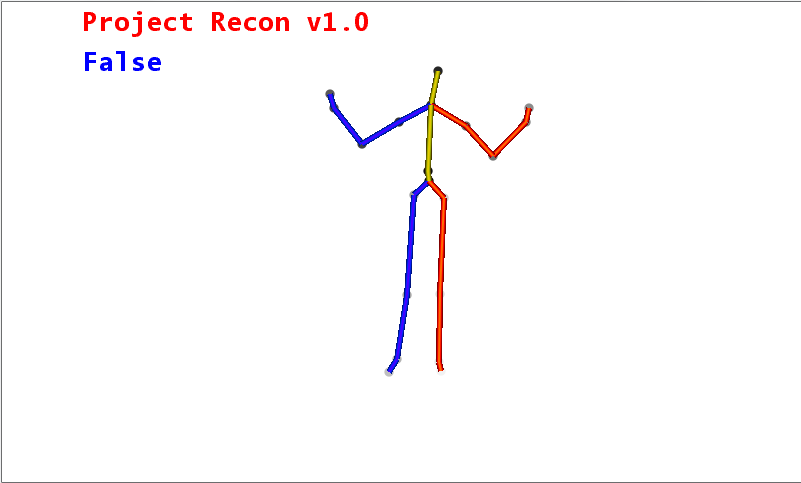
\includegraphics[scale=1]{images/skeleton_frame1.png}
\caption{initial frame}
\label{4.1}
\end{figure}
\\
\begin{figure}[ht]
\centering
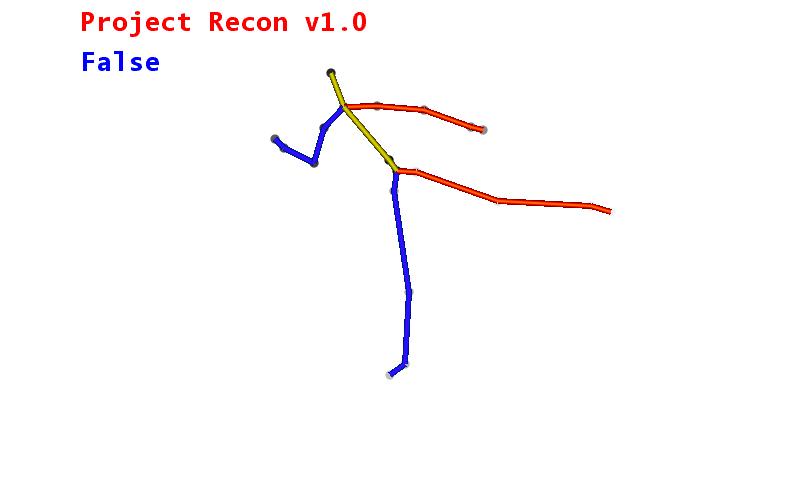
\includegraphics[scale=1]{images/skeleton_frame2.png}
\caption{few seconds later from initial frame}
\label{4.2}
\end{figure}

\subsection{Kinect}
What makes Kinect sensor a good choice for this project is its ability to recognize and keep track of a person's movement through creating a virtual skeleton that matches the user and makes the skeleton move with the user. There are few constraints unfortunately when it comes to incorporating it with the Jiu Jitsu training. One of which would be the fact that Kinect does not differentiate between a user who is facing the Kinect from a user who is giving his back to the Kinect sensor.
\\
\\
The Kinect sensor consists of three major parts. A regular camera used mostly for video chat on the XBox and the Kinect and sometimes visualization (e.g adding the user inside the scene of the game). The other two major parts are the ones that detect the user and their motion. The first is an infrared emitter and the other is an infrared sensor. The way the Kinect works is that the infrared emitter emits a mesh of infrared rays that would reflect back to the Kinect off from the user and then are detected by the sensor.
\\
\\
The Kinect sensor has sends as an output three streams, an audio stream, a depth image stream and a color image stream. In the image below the color image stream is used to render the regular image captured by the Kinect camera.
\\
\begin{figure}[ht]
\centering
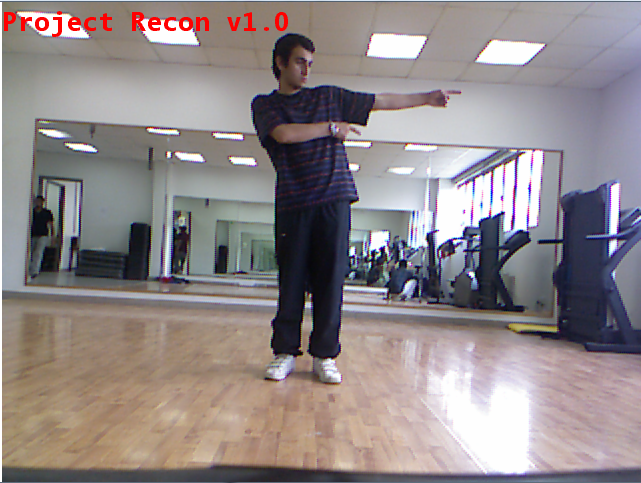
\includegraphics[scale=1]{images/color_data.png}
\caption{Color stream data visualization}
\label{4.3}
\end{figure}
\\
\\
Other streams that the Kinect provides as output are the skeleton stream, Kinect provides an array of skeletons (having skeletons of all available users). So far the array has a maximum of four users at a time. The skeleton stream can be used to acquire information regarding the skeleton of a certain user. In the next image, a circle was used to identify the places of the joints and was drawn on its respective joint. Different shades of grey were used in this image to show the system's differentiation of the joints.
\\
\begin{figure}[ht]
\centering
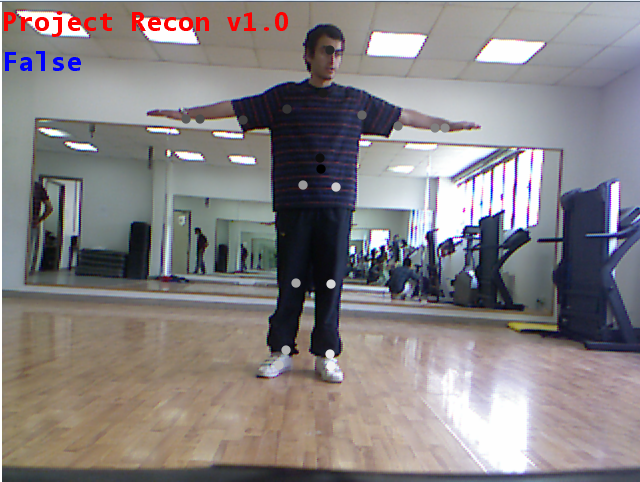
\includegraphics[scale=1]{images/color_joints.png}
\caption{Color stream data visualization with a visualization of the joints that is provided from the skeleton stream}
\label{4.4}
\end{figure}
\\
There is a total of 20 joints recognized by the Kinect sensor. The head, the center shoulder, right shoulder, left shoulder, right and left elbows, right and left wrists, right and left hands, right and left hips, right and left knees, right and left ankles, right and left feet, a center hip and a spine.
\\
\\
After visualizing the joints, the next step was to link the joints with a line to show the skeleton itself. By simple line equations and using the two points as the joints, the skeleton was drawn in the following manner:
\\
\\
%\includefig{color_skeleton.png}
\begin{figure}[ht]
\centering
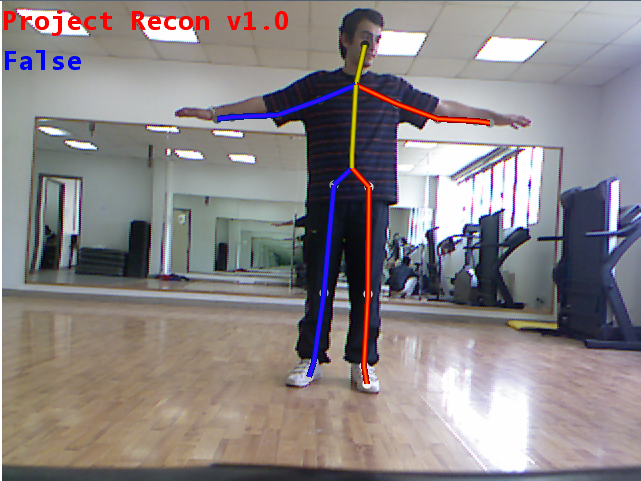
\includegraphics[scale=1]{images/color_skeleton.png}
\caption{Color stream data visualization and skeleton visualization}
\label{4.5}
\end{figure}
%\centerline{fig.4.5 (Color stream data visualization and skeleton visualization)}
\\
\\

%here discuss that there are different space systems
Kinect uses three different coordinate systems. Each one is different to the other, however have relations to one another. Those spaces are Skeleton Space, Color Space and Depth Space. Kinect streams information on those three spaces during each frame.
%Color Space
\\
\\
The Color Space is a 2D space having only X and Y as its coordinates. During each frame, the color sensor (camera) captures an image of everything in the visibility box of the camera itself. The frame of the Color Space is made up of pixels, where the size is determined by the specified NUI\_IMAGE\_RESOLUTION. Resolution could be either 80 x 60, 320 x 240, 640 x 480, or 1280 x 960. Every pixel contains the three values of red, green and blue at the particular coordinate.

%Picture of a Color Space here

%Depth Space
Similar to the Color Space, the Depth Space is a 2D space with X and Y as its coordinates. Each frame is represented as a gray scale image of the visibil objects to the camera. The frame size is also determined by the specified NUI\_IMAGE\_RESOLUTION, where each pixel contains the Cartesian distance between the camera plane and the nearest body. The distance is measured in millimeters.


%Skeleton Space
\subsection{Connections and Communications}
The communication between Project Recon and the interface is seen as a client-server communication. When browsing the possible technologies to use, socket programming came at the top of the list.
\\
\\
Socket Programming uses the client server model of network communication, in which a server (in this case the interface) would listen on different ports for data arriving from any of the devices that are supposed to connect to it. When Project Recon starts and is ready it will take the part of the client, as it will send its data stream to the specified socket. When ready, a handshake will occur to initialize connection between starting to send the data stream. In which the interface will receive the data of gestures and delivers the proper output.
\\
\\
There are three different data streams, a data stream responsible for system-related gestures, like a gesture to start the session or end it. The other stream consists of technique details. Finally, the third stream is contains the impact of the technique. All of the three streams have a timestamp in order to associate each impact with the proper technique used.

%Project Fast in Recognition in real time
%Robust and Dynamic in terms of Motion Recognition
%Be able to plugin to different systems
%be able to send data to the interface ad monitor in order to make it visibe to the user playing

\section{Project Requirements}
%In order to ensure best performance, certain constraints need to be handled. 
The practice that is targeted by the project is fast paced, which means the system needs to be performant enough to handle fast motion and recognize the technique in real time. Also, for it being a dynamic practice, which means rapid movement takes place during practice and the user will not necessiraly be always facing the Kinect as he will be moving freely around the practice room and most of the times will be giving his back to the Kinect. We need to make the system robust enough to be able to recognize different motions.
\\
\\
Another basic requirement is to allow the differentiation between two different users infront of the Kinect, one being the coach and the second being the practitioner. This is easily resolved as Kinect's stream sends multiple skeletons of the multiple users. However it is required that the first user be defined as a the practitioner and the second to join in later would be the coach.
\\
\\
Finally, the project should be able to plugin to a different system, the fitness monitor. The fitness monitor is an interface that shows the user's current stats, technique executed, and more. A connection should be established between Project Recon and the fitness monitor, where Project Recon should be able to send information regarding the technique executed by the user for the fitnes monitor display.